\documentclass[11pt]{beamer}
%\usefonttheme{professionalfonts}
\usefonttheme{serif}

\usepackage[utf8]{inputenc}
\usepackage[T1]{fontenc}
\usepackage{lmodern}
\usepackage[spanish]{babel}
\usepackage{amsmath}
\usepackage{amssymb}
\usepackage{cancel}
\usetheme{EastLansing}
\usepackage{graphicx}
\usepackage[]{xcolor}
\usepackage{tikz}
%\usepackage[table]{xcolor}
\usepackage{colortbl}
\usetikzlibrary{shapes.geometric, arrows}

\author{Dr. Alejandro Rodriguez}
\title{Probabilidad y Estad\'istica\\Probabilidad}
\subtitle{Universidad Tecnol\'ogica Iz\'ucar de Matamoros\\UTIM }


\begin{document}

    \begin{frame}[plain]
        \maketitle
    \end{frame}

    \begin{frame}{Temas de Probabilidad}
      \begin{itemize}
          \item Conjuntos
          \item Probabilidad Básica y Condicional
          \item Distribuciones Discretas de Probabilidad
          \item Distribuciones Continuas de Probabilidad
          \item Distribuciones Muestrales
      \end{itemize}
    \end{frame}
    \begin{frame}{Probabilidad}
       \begin{block}{Probabilidad}
           El término \textbf{probabilidad} se refiere al estudio de azar y la incertidumbre en cualquier
           situación en la cual varios posibles sucesos pueden ocurrir.
       \end{block}
       \pause
       En palabras simples, fenómenos aleatorios son los que pueden dar lugar a varios resultados, sin que pueda ser posible enunciar con certeza cuál de éstos va a ser observado en la realización del experimento.
    \end{frame}



    \section*{Conjuntos}
      \begin{frame}{Espacio muestral}
          \begin{block}{title}
              Definir los conceptos y notación de conjuntos:
              -Universo
              -Vacío
              -Subconjunto

              Describir el proceso de construcción del diagrama de Venn Euler.

              Explicar las operaciones entre conjuntos:
              - Unión
              - Intersección
              - Complemento
              - Diferencia
          \end{block}
      \end{frame}
      \subsection*{Espacio Muestral}
        \begin{frame}{Conjuntos o espacio muestral}
          \begin{block}{Espacio muestral}
              El \textbf{espacio muestral} de un experimento denotado por $E$ , es el \textbf{conjunto} de todos los posibles resultados de dicho experimento.
          \end{block}
          \pause
          Ejemplos:
          \begin{enumerate}[<+->]
              \item El espacio muestral asociado a lanzar un dado, E = {1,2,3,4,5,6}
              \item El espacio asociado a preguntar a un cliente si le gusta o no nuestro producto es E ={S, N} (S – sí; N – no)
              \item El espacio asociado a indagar si 3 clientes que entraron a una tienda compraron un producto es E = {SSS, SSN, SNS, NSS, SNN, NSN, NNS, NNN}.
          \end{enumerate}
        \end{frame}
      \subsection*{Suceso o evento}
        \begin{frame}{Conjuntos: Suceso o evento}
          \begin{block}{Suceso o evento}
              Un \textbf{suceso} o \textbf{evento} es cualquier recopilación (\textbf{subconjunto}) de resultados contenidos en el espacio muestral $E$. Un evento es \textit{simple} si consiste en exactamente un resultado y \textit{compuesto} si consiste en más de un resultado.
          \end{block}
          \pause
          Dado que los sucesos son subconjuntos del espacio muestral, son muy útiles los diagramas de Venn para su representación:
          \begin{figure}
              \centering
              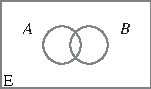
\includegraphics[width=0.3\linewidth]{images/estadistica1}
              \caption{Ejemplo de un diagrama de diagramas de Venn. E. Espacio muestral, A y B representan conjuntos o subconjuntos. }
              \label{fig:estadistica1}
          \end{figure}
        \end{frame}
      \subsection*{Propiedades de conjunto}
        \begin{frame}{}
          \begin{block}{Propiedades de conjunto}
              \begin{enumerate}[<+->]
                  \item El complemento de un evento A, denotado por A', es el conjunto de todos los resultados en \textbf{E} que no están contenidos en A.
                  \item La unión de dos eventos A y B, denotados por A $\cup$ B y leídos “A o B”, es el evento que consiste en todos los resultados que están en A o en B o en ambos eventos (de tal suerte que la unión incluya resultados donde tanto A como B ocurren, así también resultados donde ocurre exactamente uno), es decir, todos los resultados en por lo menos uno de los eventos.
                  \item La intersección de dos eventos A y B, denotada por A $\cap$ B y leída “A y B”, es el evento que consiste en todos los resultados que están tanto en A como en B.
              \end{enumerate}
          \end{block}
        \end{frame}

        \begin{frame}{Unión}
          \begin{figure}
              \centering
              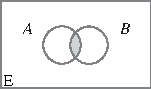
\includegraphics[width=0.7\linewidth]{images/estadistica2}
              \caption{Unión: La región sombreada es A $\cup$ B.}
              \label{fig:estadistica2}
          \end{figure}

        \end{frame}
        \begin{frame}{Intersección}
          \begin{figure}
            \centering
            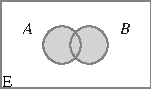
\includegraphics[width=0.7\linewidth]{images/estadistica3}
            \caption{Intersección: La región sombreada es A $\cap$ B}
            \label{fig:estadistica3}
          \end{figure}

        \end{frame}
        \begin{frame}{Complemento}
          \begin{figure}
            \centering
            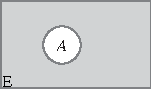
\includegraphics[width=0.7\linewidth]{images/estadistica4}
            \caption{Complemento: La región sombreada es A'. }
            \label{fig:estadistica4}
          \end{figure}

        \end{frame}
        \begin{frame}{Mutuamente excluyentes}
        \begin{figure}
            \centering
            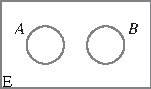
\includegraphics[width=0.7\linewidth]{images/estadistica5}
            \caption{Eventos mutuamente
excluyentes.}
            \label{fig:estadistica5}
        \end{figure}

      \end{frame}

        \begin{frame}{Mutuamente excluyentes}
           \textbf{\begin{center}
                 \huge TO BE CONTINUE
        \end{center}}
        \end{frame}


    \section*{Probabilidad Básica y Condicional}
      \subsection*{Métodos para el cálculo de probabilidad}
        \begin{frame}{Probabilidad}
            \begin{block}{Probabilidad}
                El término \textbf{probabilidad} se refiere al estudio de azar y la incertidumbre en cualquier
                situación en la cual varios posibles sucesos pueden ocurrir.
            \end{block}

            En palabras simples, fenómenos aleatorios son los que pueden dar lugar a varios resultados, sin que pueda ser posible enunciar con certeza cuál de éstos va a ser observado en la realización del experimento.
        \end{frame}

        \begin{frame}{}
            \begin{center}
                \textbf{\huge Cálculo de probabilidad}
            \end{center}
        \end{frame}

        \begin{frame}{Cálculo de probabilidad}
            La noción de probabilidad tiene cuatro acepciones básicas:
            \\
            \begin{itemize}[]
                \item Empírica (práctica, relacionada con la frecuencia relativa)
                \item Clásica (teórica, relacionada con casos equiprobables)
                \item Axiomática (basada en un modelo matemático)
                \item Intuitiva (relacionada con experiencias o mediciones subjetivas)
            \end{itemize}
        \end{frame}






        \subsubsection*{Método Empírico}
          \begin{frame}{Método empírico}
            J. J. Bernoulli, observando los resultados del lanzamiento de una moneda un número grande de veces, notó que el número de caras y cruces tendía a igualarse. Es decir, que la frecuencia relativa de la obtención de caras se acercaba más al número de cruces, cuanto mayor era el número de lanzamientos, dicho de otra manera, las frecuencias relativas se parecían cada vez más a 0.5. De aquí la definición empírica de Probabilidad:
            \begin{block}{Probabilidad}
               \textbf{Probabilidad} de un suceso es el número al que tiende la frecuencia relativa asociada al suceso a medida que el número de veces que se realiza el experimento crece.
               $$P(A) = \lim_{N \to \infty }\dfrac{n(A)}{N} $$
            \end{block}
          \end{frame}


           \begin{frame}{Método empírico}
               \begin{block}{Ejemplo}
                   En una línea de envasado de cereales se tienen los siguientes registros de envases defectuosos:
                   \begin{table}[!h]
                       \centering
                       \begin{tabular}{|c|c|c|c|c|c|}
                           \hline
                           Semana & 1 & 2 & 3 & 4 & Total\\
                           \hline
                           Envases recibidos  & 1200 & 1350 & 1150 & 1100 & 4800\\
                           Envases rechazados & 4    & 6    & 4    & 5    & 19\\
                           \hline
                       \end{tabular}
                   \end{table}
                   Determine la probabilidad de encontrar un envase defectuoso.
               \end{block}
               \pause
               \textbf{Solución:}\\
               Evidentemente la frecuencia relativa de ocurrencia de este suceso es igual a $19/4800 = 0.004$ o lo que es lo mismo de un 0.4\%.
           \end{frame}



        \subsubsection*{Método Clásico}


          \begin{frame}{Probabilidad Clásica (Definición de Laplace)}
            \begin{block}{Enfoque clasico}
               Es el \textbf{\textit{número de casos favorables al evento}} (es decir, resultados posibles del evento o prueba que hacen que ocurra el evento) \textit{\textbf{entre el número de casos posibles}} (o sea todos los resultados posibles del experimento), \textit{\textbf{pero considerando que cada uno de los casos posibles tiene igual probabilidad de ocurrir}}.
               $$P(E) = \dfrac{n(E)}{N}$$
               $n(E)$: número de casos favorables a E\\
               $N$: número de casos posibles
            \end{block}
          \end{frame}

         \begin{frame}{Probabilidad Clásica (Definición de Laplace). Ejemplo}
             Ejemplo: El evento que consiste en obtener un mismo número de ambos dados al lanzar dos dados tiene probabilidad
             $$P(E) = \dfrac{6}{36} = \dfrac{1}{6}$$
             \pause
             \begin{table}[!h]
               \centering
               \begin{tabular}{|c|c|c|c|c|c|}
                   \hline
                   \cellcolor{blue!25} 11 & 21 & 31 & 41 & 51 & 61 \\
                   \hline
                   12 & \cellcolor{blue!25} 22 & 32 & 42 & 52 & 62 \\
                   \hline
                   13 & 23 & \cellcolor{blue!25} 33 & 43 & 53 & 63 \\
                   \hline
                   14 & 24 & 34 & \cellcolor{blue!25} 44 & 54 & 64 \\
                   \hline
                   15 & 25 & 35 & 45 & \cellcolor{blue!25} 55 & 65 \\
                   \hline
                   16 & 26 & 36 & 46 & 56 & \cellcolor{blue!25} 66 \\
                   \hline
               \end{tabular}
             \end{table}
             \begin{center}
                 Combinaciones: 36
             \end{center}
         \end{frame}





        \subsubsection*{Método Subjetivo o Intuitivo}
          \begin{frame}{Método Subjetivo o Intuitivo}
            Hay otro tipo de probabilidades como la llamada probabilidad \textbf{subjetiva} o \textbf{intuitiva} que es una cierta evaluación personal de la probabilidad, en lugar de ser teórica o experimental. Por ejemplo, si se desea opinar acerca de las posibilidades de que llueva en mayo en Izúcar de Matamoros, uno puede opinar, de acuerdo a la experiencia propia, acorde con los años en que ha residido en un lugar, por ejemplo que mañana es posible que la probabilidad de lluvia sea de un 20 \%, muy distinta a la que pudiera decir la misma persona si le preguntan en junio, un mes en el que comienzan las lluvias por esta región de Izúcar. No obstante, en ciertos estudios y situaciones los criterios de los expertos pueden utilizarse y manejarse incluso utilizando métodos estadísticos.
          \end{frame}

      \subsection*{Técnicas de conteo}

        \begin{frame}{}
           \begin{center}
               \textbf{\huge Técnicas de conteo}
           \end{center}
        \end{frame}

        \begin{frame}{Técnicas de conteo}
            Para utilizar el enfoque clásico de la probabilidad (a priori), es necesario conocer el numero total de resultados de una muestra o experimento.

            Las \textbf{técnicas de conteo} generalmente se utilizan como un medio para determinar el número total de resultados y son empleadas cuando realizar el conteo de forma manual se hace complicado.
            \pause
            \begin{block}{Técnicas de conteo}
                Las \textbf{Técnicas de conteo} son una serie de métodos de probabilidad para contar el número posible de arreglos dentro de un conjunto o varios conjuntos de objetos
            \end{block}
            \begin{itemize}
                \item Diagrama de Árbol
                \item Regla multiplicativa
                \item Permutación
                \item Combinación
            \end{itemize}
        \end{frame}



        \subsubsection*{Diagrama de Árbol}
          \begin{frame}{Diagrama de Árbol}
            Un diagrama de árbol es una representación gráfica de los posibles resultados de un experimento que tiene varios pasos.
            \begin{figure}
                \centering
                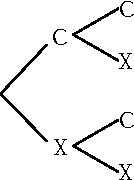
\includegraphics[width=0.3\linewidth]{images/estadistica6}
                \caption{Lanzamiento de una monada, dos veces consecutivas.}
                \label{fig:estadistica6}
            \end{figure}

          \end{frame}
          \begin{frame}{Diagrama de Árbol}
              \begin{figure}
                  \centering
                  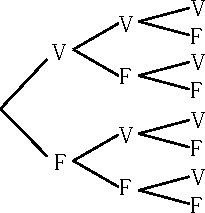
\includegraphics[width=0.3\linewidth]{images/estadistica7}
                  \caption{Posibles respuestas  de V o F, en un examen de tres preguntas.}
                  \label{fig:estadistica7}
              \end{figure}

          \end{frame}
        \subsubsection*{Regla multiplicativa}
          \begin{frame}{Regla multiplicativa}
            \begin{block}{Regla multiplicativa}
                Si una operación puede realizarse en $n_i$ formas, y si por cada una de éstas una segunda operación puede llevarse a cabo en $n_2$ formas, entonces las dos operaciones pueden realizarse juntas en $n_1n_2$ formas.
            \end{block}
            \begin{block}{Ejemplo}
                ¿Cuantos puntos muetrales hay en una espacio muestral cuando se lanza un par de dados una sola vez?
                \pause
                \textbf{Solución}: El primer dado puede caer en cualquiera de $n_1 = 6$ formas. Para cada una de éstas el segundo puede, también, caer en $n_2 = 6$ formas. Por tanto el par de dados pueden caer:
                $$ n_1n_2 = (6)(6) = 36 $$
            \end{block}
          \end{frame}



        \subsubsection*{Permutación y Combinación}
          \begin{frame}{Definición de Factorial!}
            \begin{block}{Definición de Factorial!}
                El \textbf{factorial de un entero positivo} $n$ se define como el producto de todos los números enteros positivos desde 1 hasta n. \\Por ejemplo:

               $$ 5!=1\times 2\times 3\times 4\times 5=120.$$

            \end{block}
            \begin{block}{Propiedades del de Factorial!}
                $$ 0! = 1$$
                $$ (1 + 4)! = 5! = 120$$
                $$ (6 - 2)! = 4! = 24$$

            \end{block}
          \end{frame}

          \begin{frame}{Propiedades del de Factorial!}

            \begin{block}{Propiedades del de Factorial!}
               $$\dfrac{5!}{7!} = \dfrac{5 \times 4 \times 3 \times 2 \times 1}{7 \times 6 \times 5 \times 4 \times 3 \times 2 \times 1} = \dfrac{\cancel{5!}}{7 \times 6 \times \cancel{5!}} = \dfrac{1}{7 \times 6} = \dfrac{1}{42}$$
               Otro ejemplo:\\
               \pause
               $$\dfrac{4!}{2!} = \dfrac{4 \times 3 \times 2 \times 1}{2 \times 1} = \dfrac{4 \times 3 \times \cancel{2!}}{\cancel{2!}} = 4 \times 3 = 12$$
            \end{block}
          \end{frame}

          \begin{frame}{Permutación y Combinación}
              Considérese un grupo de \textbf{\textit{n}}\textbf{ individuos u objetos distintos}.

              - ¿Cuántas maneras existen de seleccionar un subconjunto de tamaño k del grupo?\\
              \pause
              \begin{block}{Ejemplos}
                 \begin{itemize}
                     \item Si un equipo de ligas menores tiene 15 jugadores registrados, ¿cuántas maneras existen de seleccionar 9 jugadores para una alineación inicial?
                     \item Si en su librero tiene 10 libros de misterio no leídos y desea seleccionar 3 para llevarlos consigo en unas vacaciones cortas, ¿cuántas maneras existen de hacerlo?
                 \end{itemize}
              \end{block}
          \end{frame}

          \begin{frame}{Permutación y Combinación}
              Una respuesta a la pregunta general que se acaba de plantear requiere distinguir entre
dos casos.
              \begin{itemize}
                  \item El orden de selección importa.
                  \item El orden de selección \textbf{NO} importa.
              \end{itemize}

              \pause
              \begin{block}{Ejemplos}
                  \begin{itemize}
                      \item Con Jorge como lanzador y Daniela como receptor se obtiene una
alineación diferente de aquella con Daniela como receptor y Jorge como lanzador.
                      \item La selección del libro que va a leer no es importante.
                  \end{itemize}
              \end{block}

          \end{frame}

         \begin{frame}{Permutación y Combinación. Definición.}
           \begin{block}{Definici\'on}
               \underline{Un subconjunto ordenado se llama \textbf{permutación}}. El número de permutaciones de tamaño $k$ que se puede formar con los $n$ individuos u objetos en un grupo será denotado por $P_{k,n}$.\\
               \pause
               \underline{Un subconjunto no ordenado se llama \textbf{combinación}}. Una forma de denotar el
número de combinaciones es $C_ {k,n}$, pero en su lugar se utilizará una notación que es bastante común en libros de probabilidad:$\binom{n}{k}$, que se lee “\textit{de n se eligen k}”.
           \end{block}
         \end{frame}

         \begin{frame}{Permutación}
           \begin{block}{Ejemplo}
               Supongamos que tenemos un conjunto de cuatro individuos: \textit{a}, \textit{b}, \textit{c} y \textit{d}. De ellos solo dos van a ser elegidos para los puestos de \textit{presidente} y \textit{vicepresidente} en cierta junta directiva.\\
               ¿Cuantas maneras exciten para seleccionar estos dos cargos?
           \end{block}
           \pause

           \begin{center}
               \begin{tabular}{ccc}
               ab & ac & ad \\
               ba & bc & bd \\
               ca & cb & cd \\
               da & db & dc \\
           \end{tabular}
           \end{center}
           Total: 12 formas.\\
           NOTA: Uno esta tentado a decir combinaciones sin embargo, el orden importa, por lo que son \textbf{permutaciones}.
         \end{frame}

         \begin{frame}{Permutación}
             \begin{block}{Ejemplo}
                 Supongamos que tenemos un conjunto de cuatro individuos: \textit{a}, \textit{b}, \textit{c} y \textit{d}. De ellos solo dos van a ser elegidos para los puestos de \textit{presidente} y \textit{vicepresidente} en cierta junta directiva.\\
                 ¿Cuantas maneras exciten para seleccionar estos dos cargos?
             \end{block}
             \pause
             \begin{center}
                 \begin{tabular}{ccc}
                     ab & ac & ad \\
                     ba & bc & bd \\
                     ca & cb & cd \\
                     da & db & dc \\
                 \end{tabular}
             \end{center}
             $$P_{k,n}=\dfrac{n!}{(n-k)!}$$
             $$P_{k,n}=\dfrac{n!}{(n-k)!}=\dfrac{4!}{(4-2)!}=\dfrac{4 \times 3 \times \cancel{2!}}{\cancel{2!}}= 4 \times 3 = 12$$
         \end{frame}


         \begin{frame}{Permutación. Ejemplo}
             \begin{block}{Ejemplo}
               Existen diez asistentes de profesor disponibles para calificar exámenes en un curso. El examen se compone de cuatro preguntas y el
profesor desea seleccionar un asistente diferente para calificar cada pregunta (sólo un asistente por pregunta). ¿De cuántas maneras se pueden elegir los asistentes para calificar?
             \end{block}
             \pause
             n $=$ tamaño del grupo $=$ 10\\
             k $=$ tamaño del subconjunto $=$ 4\\
             $$P_{k,n}=\dfrac{n!}{(n-k)!} = \dfrac{10!}{(10-4)!}= \dfrac{10 \times 9 \times 8 \times 7 \times 6!}{6!}=$$
             \pause
             $$= \dfrac{10 \times 9 \times 8 \times 7 \times \cancel{6!}}{\cancel{6!}}= 10 \times 9 \times 8 \times 7= 5040$$
         \end{frame}

         \begin{frame}{}
             \begin{center}
                 \textbf{\huge Técnicas de conteo\\  Combinación}
             \end{center}
         \end{frame}

         \begin{frame}{Combinación}
             \begin{block}{Definici\'on}
                 \underline{Un subconjunto no ordenado se llama \textbf{combinación}}. Una forma de denotar el número de combinaciones es $C_ {k,n}$, pero en su lugar se utilizará una notación que es bastante común en libros de probabilidad:$\binom{n}{k}$, que se lee “\textit{de n se eligen k}”.
             \end{block}
             \pause
             Considérense ahora las combinaciones (es decir, subconjuntos ordenados). Tomando el ejemplo anterior, el de los cuatro individuos\\ \begin{center}
                 \textit{a}, \textit{b}, \textit{c} y \textit{d}.
             \end{center}
         Supóngase que dos de los cuatro individuos tienen que ser seleccionados para que asistan a una conferencia. El orden de selección no es importante; lo que importa es cuáles dos son seleccionados.

         \end{frame}

         \begin{frame}{Combinación}
            Considérense ahora las combinaciones (es decir, subconjuntos ordenados). Tomando el ejemplo anterior, el de los cuatro individuos\\ \begin{center}
                 \textit{a}, \textit{b}, \textit{c} y \textit{d}.
             \end{center}
             Supóngase que dos de los cuatro individuos tienen que ser seleccionados para que asistan a una conferencia. El orden de selección no es importante; lo que importa es cuáles dos son seleccionados.

             Nos percatamos que el orden de selección no es importante, da lo mismo seleccionar a \textit{\textbf{ab}} que a \textit{\textbf{ba}}.
             \begin{center}
                 ab $\Leftrightarrow$ ba
             \end{center}
             \begin{center}
                 ab, ac, ad, bc, bd, cd
             \end{center}
         \end{frame}

         \begin{frame}{Combinación}
             \begin{block}{Combinación}
               $$\binom{n}{k} = \dfrac{P_{k,n}}{k!} = \dfrac{n!}{k!(n-k)!} $$
             \end{block}
             Del ejemplo anterior tenemos:
             $$\binom{n}{k} = \dfrac{n!}{k!(n-k)!} = \dfrac{4!}{2!(4-2)!}= \dfrac{4 \times 3 \times 2!}{2! \times 2!}=\dfrac{4 \times 3 \times \cancel{2!}}{2! \times \cancel{2!}}=$$
             $$\dfrac{4 \times 3}{2} = 12/2 = 6$$
             \pause

             \begin{center}
                 ab, ac, ad, bc, bd, cd
             \end{center}
         \end{frame}


      \subsection*{Conceptos de probabilidad}
        \begin{frame}{Combinación}
          \textbf{\begin{center}
                   \huge Conceptos de probabilidad
          \end{center}}
        \end{frame}

        \begin{frame}{Probabilidad Condicionada}
          En numerosas ocasiones, tendremos que modelar una situación en la que se dispone de información adicional, \textbf{debiendo condicionarse a sucesos o circunstancias}. Supongamos que estamos interesados en un suceso A; hemos asignado P(A) y nos informan que ha ocurrido el suceso B y queremos saber cómo cambian mis creencias sobre A.
          \pause
          \begin{block}{Probabilidad Condicionada}
            Para dos eventos cualesquiera A y B con $P(B) >  0$, la \textbf{probabilidad condicional de A dado que B ha ocurrido} está definida por:
            $$ P(A|B)=\dfrac{P(A\cap B)}{P(B)}$$
          \end{block}

        \end{frame}

        \begin{frame}{Probabilidad Condicionada}

            \begin{block}{Probabilidad Condicionada. Ejemplo}
                Calcular la probabilidad de obtener un 6 al tirar un dado sabiendo que ha salido par.
             \end{block}
            \pause
            \begin{block}{}
                $$P(A)= \pause \dfrac{1}{6} $$\\

                $$P(B)= \pause \dfrac{3}{6}$$
                $$P(A\cap B) = \pause \dfrac{1}{6}$$\\

                $$ P(A|B)=\dfrac{P(A\cap B)}{P(B)} = \pause \dfrac{\dfrac{1}{6}}{\dfrac{3}{6}}=\dfrac{1}{3}$$
            \end{block}
        \end{frame}

        \begin{frame}{Ejemplo de la tienda de cámaras.}
            \begin{block}{Ejemplo de la tienda de cámaras.}
              Supóngase que de todos los individuos que compran cierta cámara digital, 60\% incluye
una tarjeta de memoria opcional en su compra, 40\% incluyen una batería extra y 30\% incluyen tanto una tarjeta como una batería. \\

              Considere seleccionar al azar un comprador y sea A = {tarjeta de memoria adquirida} y B = {batería adquirida}
              Dado que el individuo seleccionado adquirió una batería extra, ¿cual es la probabilidad de haber adquirido una tarjeta opcional?
            \end{block}
            \begin{block}{Solución}
               \begin{itemize}
                   \item P(A) = \pause 0.60
                   \item P(B) = \pause 0.40
                   \item P(ambas adquiridas) = \pause P(A $\cap$ B) = 0.30
               \end{itemize}
            \end{block}
        \end{frame}

        \begin{frame}{Ejemplo de la tienda de cámaras.}

            \begin{block}{Solución}
                \begin{itemize}
                    \item P(A) = \pause 0.60
                    \item P(B) = \pause 0.40
                    \item P(ambas adquiridas) = \pause P(A $\cap$ B) = 0.30
                \end{itemize}

            \end{block}
            \pause
            $$P(A|B)=\dfrac{P(A\cap B)}{P(B)} = \dfrac{0.3}{0.4} = 0.75 $$
            Es decir, de todos los que adquieren una batería extra, 75\% adquirieron una tarjeta de memoria opcional.
        \end{frame}

        \begin{frame}{Probabilidad Incondicionada}
          ¿Que sucede cuando los eventos son independientes entre si?\\
          \pause
          \begin{block}{Probabilidad Incondicionada}
                      Dos sucesos, A y B, son independientes cuando la probabilidad de que suceda A no se ve afectada porque haya sucedido, o no, B.
          \end{block}
          Por ejemplo: Si lanzamos dos veces una moneda, el segundo resultado que obtengamos no estará influenciado por el primer resultado obtenido.\\
          Como lo calculamos:
          \pause
          \begin{block}{Probabilidad Incondicionada}
            $$ P(A|B)=\dfrac{P(A)P(B)}{P(B)}=P(A)$$
            $$ P(A|B)=P(A)$$
          \end{block}
    \end{frame}


    \section*{Distribuciones Probabilidad}
      \begin{frame}{}
          \begin{center}
              \textbf{\huge Distribuciones de Probabilidad}
          \end{center}
      \end{frame}


      \begin{frame}{Distribuciones de Probabilidad}
          \begin{itemize}
              \item Distribuciones Discretas de Probabilidad
              \item Distribuciones Continuas de Probabilidad
              \item Distribuciones Muestrales*
          \end{itemize}
      \end{frame}

      \subsection*{Distribuciones Probabilidad}
        \begin{frame}{Distribuciones de Probabilidad}
            \begin{block}{Recordando}
              El \textbf{espacio muestral} \pause es el conjunto de resultados posibles del experimento aleatorio. Hay una gran variedad de experimentos aleatorios que nos pueden dar resultados tan diversos como: para lanzar una moneda  \textit{{sol ; águila}}; para lanzar un dado  \textit{{1, 2, 3, 4, 5, 6}}; para ver si una unidad cumple o no cumple especificaciones \textit{{pasa, no pasa}}; ver el pH de una muestra de agua \textit{{todo el conjunto de valores entre 6 y 9 digamos}}; etc. \\
              \pause
              Esto quiere decir que de los experimentos aleatorios podemos obtener números, textos, valores booleanos (binarios), etc. En correspondencia tendremos variables aleatorias del mismo carácter.\\
            \end{block}
        \end{frame}


        \begin{frame}{Distribuciones de Probabilidad}
            \begin{block}{Ampliando el concepto previo de variables.}
                \begin{itemize}
                    \item \textbf{Variable aleatoria discreta:} Puede tomar una cantidad finita de valores o infinita pero numerable. Esto quiere decir que sus valores son un número finito de números reales distintos.
                    \item  \textbf{Variable aleatoria continua:} La cantidad de valores que puede adoptar es una cantidad infinita. Esto quiere decir que sus valores son un intervalo o una unión de intervalos sobre la recta de los números reales.
                \end{itemize}
            \end{block}
            \begin{figure}
                \centering
                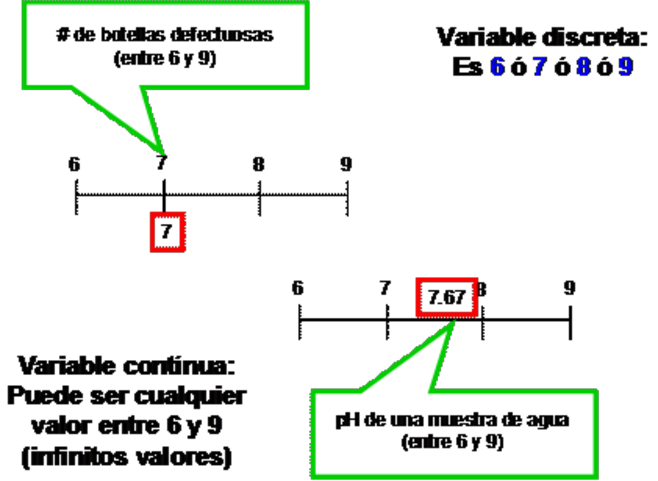
\includegraphics[width=0.3\linewidth]{images/estadistica8}
                \label{fig:estadistica8}
            \end{figure}

        \end{frame}

        \subsubsection*{Función de densidad de probabilidad}
        \begin{frame}{Función de densidad de probabilidad}
            \begin{itemize}
                \item En general, cada uno de los valores posibles de una variable aleatoria puede tener una probabilidad distinta a los demás. Al conjunto de valores posibles, y la relación entre ellos y sus respectivas probabilidades, se lo conoce como distribución de probabilidad.
                \item Las distribuciones de probabilidad pueden representarse a través de una tabla, una gráfica o una fórmula, en cuyo caso a tal regla de correspondencia se le denomina \textbf{función de densidad de probabilidad}.
            \end{itemize}
            \begin{block}{Propiedades}
                \begin{itemize}
                    \item Que no puede ser negativa en ningún punto
                    \item La suma de las probabilidades de todos los valores posibles es igual a 1.
                \end{itemize}
            \end{block}
        \end{frame}

        \begin{frame}{Función de densidad de probabilidad}
          \begin{block}{Ejemplo}
             Consideremos a la variable aleatoria X como suma de los valores que se obtienen al lanzar un dado 2 veces. El espacio muestral es el conjunto {2,3,4,5,6,7,8,9,10,11,12}.
          \end{block}
          \pause
          \begin{center}
              \begin{tabular}{c|cccccc}
                 i;j & 1 & 2 & 3 & 4 & 5 & 6 \\
                  \hline
                  1 & 2 & 3 & 4 & 5 & 6 & 7 \\
                  2 & 3 & 4 & 5 & 6 & 7 & 8 \\
                  3 & 4 & 5 & 6 & 7 & 8 & 9 \\
                  4 & 5 & 6 & 7 & 8 & 9 & 10 \\
                  5 & 6 & 7 & 8 & 9 & 10 & 11 \\
                  6 & 7 & 8 & 9 & 10 & 11 & 12 \\
              \end{tabular}
          \end{center}
        \end{frame}

        \begin{frame}{Función de densidad de probabilidad}
            Vea la tabla donde se expone la probabilidad asociada a cada valor y su histograma.
            \begin{columns}
                \begin{column}{0.4\textwidth}
                    \begin{center}
                        \begin{tabular}{c|c}
                            X & P(X=x)\\
                            \hline
                            2 & 0.027 \\

                            3 & 0.055 \\

                            4 & 0.083 \\

                            5 & 0.111 \\

                            6 & 0.138 \\

                            7 & 0.166 \\

                            8 & 0.138 \\

                            9 & 0.111 \\

                            10 & 0.083 \\

                            11 & 0.055 \\

                            12 & 0.027 \\
                        \end{tabular}
                    \end{center}
                \end{column}
                \begin{column}{0.56\textwidth}
                    \begin{figure}
                        \centering
                        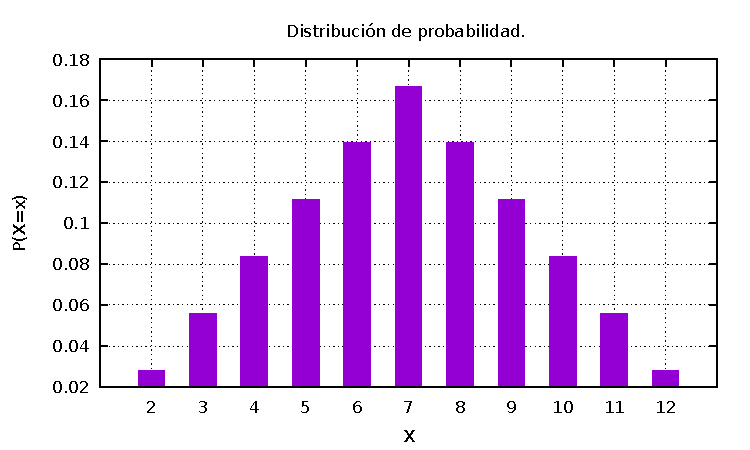
\includegraphics[width=1\linewidth]{images/p1}
                        \label{fig:p1}
                    \end{figure}
                \end{column}
            \end{columns}
        \end{frame}

      \subsection*{Distribuciones Discretas de Probabilidad}

        \begin{frame}
            \textbf{\begin{center}
                    \huge Distribuciones Discretas de Probabilidad
            \end{center}}
        \end{frame}
        \begin{frame}{Distribuciones de probabilidad de variables discretas}
          Existen varias distribuciones discretas con aplicación práctica, pero por el alcance de este curso haremos énfasis en la distribución binomial, pues tiene aplicación posterior en el Control de Calidad.
          \begin{itemize}
              \item La distribución binomial
              \item Hipergeométrica
              \item Poisson
          \end{itemize}
        \end{frame}


        \subsubsection*{La distribución binomial}
          \begin{frame}{Distribución binomial o experimento de Bernoulli}
            Existen muchos experimentos que se ajustan exacta o aproximadamente a la siguiente lista
de requerimientos:
            \begin{enumerate}
                \item El experimento consta de una secuencia de \textit{n} experimentos más pequeños llamados ensayos, donde \textit{n} se fija antes del experimento.
                \item Cada ensayo puede dar por resultado uno de los mismos dos resultados posibles, los cuales se denotan como éxito (\textbf{E}) y falla (\textbf{F}).
                \item Los ensayos son independientes, de modo que el resultado en cualquier ensayo particular no influye en el resultado de cualquier otro ensayo.
                \item La probabilidad de éxito es constante de un ensayo a otro; esta probabilidad se denota por \textbf{p}.
            \end{enumerate}
            En tal caso se tiene lo que se denomina un experimento binomial.
          \end{frame}


          \begin{frame}{Distribución binomial o experimento de Bernoulli}
              En este  experimento binomial, emplearemos las siguiente notación, el número de ensayos se denota con \textbf{n}, la probabilidad de éxito con \textbf{p} y la de fracaso con \textbf{q}.

              Hay que notar que las probabilidades de éxito y de fracaso están relacionadas de la siguiente manera: $p + q = 1.$
              La función de probabilidad es:

              $$P(X=x)=\binom{n}{x}p^xq^{n-x}=\dfrac{n!}{x!(n-x)!}p^xq^{n-x}$$
              donde
              $$x=1, 2, 3, \cdots ,n $$
          \end{frame}
          \begin{frame}{Distribución binomial. Ejemplo 1}

              \begin{block}{Ejemplo 1}
                 ¿Cuál es la probabilidad de obtener 3 águilas al lanzar una moneda 5 veces?
              \end{block}
              \begin{block}{Solución}
                 \begin{itemize}
                     \item \textbf{x} \pause es el número de éxitos, en este ejemplo igual a 3 (en cada éxito decíamos que la variable toma el valor 1, como son 3 aciertos, entonces $x = 3$)
                     \item \textbf{n} \pause es el número de ensayos. En nuestro ejemplo son 5.
                     \item \textbf{p} \pause es la probabilidad de éxito, es decir, que salga águila al lanzar la moneda. Por lo tanto $p = 0.5$.
                 \end{itemize}
                 \pause
                 $$P(X=3)=\dfrac{n!}{x!(n-x)!}p^xq^{n-x}= \pause \dfrac{5!}{3!(5-3)!}0.5^3(1-0.5)^{5-3}=0.3125\Rightarrow31.25\%$$
              \end{block}
          \end{frame}

          \begin{frame}{Distribución binomial. Ejemplo 2}
            \begin{block}{Ejemplo 2}
                De acuerdo a una encuesta, \textbf{la probabilida}d de que un cliente compre un nuevo producto que se está introduciendo en el mercado,\textbf{ es de 0.6}. Hallar la probabilidad de que al entrar \textbf{10 clientes} a una tienda \textbf{lo compren 5 clientes}. ¿Cuál será la probabilidad de que lo compren al menos 5 clientes? \\
                Grafique las probabilidades y vea como se afectan si p = 0.7.
            \end{block}
            \begin{block}{Solución}
               \begin{itemize}
                   \item \textbf{x} \pause van a ser: 5 y para la gráfica los valores del 1 al 10.
                   \item \textbf{n} \pause es el número de ensayos. En nuestro ejemplo son 10.
                   \item \textbf{p} \pause es la probabilidad de éxito, 0.6 y 0.7.
               \end{itemize}
               Calculemos la tabla de la distribución binomial con Excel.
            \end{block}
          \end{frame}

          \begin{frame}{Distribución binomial. Ejemplo 2}
              \begin{block}{Ejemplo 2}
                   Hallar la probabilidad de que al entrar \textbf{10 clientes} a una tienda \textbf{lo compren 5 clientes}. ¿Cuál será la probabilidad de que lo compren al menos 5 clientes? \\
              \end{block}

          \end{frame}
          \begin{frame}{Distribución binomial. Ejemplo 2}

              \begin{block}{Solución. Tabla}
                  \begin{center}
                      \begin{tabular}{|c|c|c|c|c|}
                      \hline
                      x &F p=0.6  &F p=0.7  &P(x)(p=0.6) &P(x)(p=0.7)   \\
                      \hline
                      0 & 0.00010 & 0.00001 & 0.00010 & 0.00001  \\
                      1 & 0.00168 & 0.00014 & 0.00157 & 0.00014  \\
                      2 & 0.01229 & 0.00159 & 0.01062 & 0.00145  \\
                      3 & 0.05476 & 0.01059 & 0.04247 & 0.00900  \\
                      4 & 0.16624 & 0.04735 & 0.11148 & 0.03676  \\
                      5 & 0.36690 & 0.15027 & 0.20066 & 0.10292  \\
                      6 & 0.61772 & 0.35039 & 0.25082 & 0.20012  \\
                      7 & 0.83271 & 0.61722 & 0.21499 & 0.26683  \\
                      8 & 0.95364 & 0.85069 & 0.12093 & 0.23347  \\
                      9 & 0.99395 & 0.97175 & 0.04031 & 0.12106  \\
                      10 & 1.00000 & 1.00000 & 0.00605 & 0.02825  \\
                      \hline
                  \end{tabular}
                  \end{center}
              \end{block}
          \end{frame}
          \begin{frame}{Distribución binomial. Ejemplo 2}

              \begin{block}{Solución}
                  La primera pregunta arroja 0.20066, o sea un 20.1 \% de probabilidad de que 5 clientes compren el producto.

                  La respuesta a la 2da pregunta es muy sencilla, es el valor de lo acumulado hasta 5 clientes que es 0.3669, o sea un 36.7\%.
              \end{block}
              \vspace{-0.23cm}
                  \begin{figure}
                      \centering
                      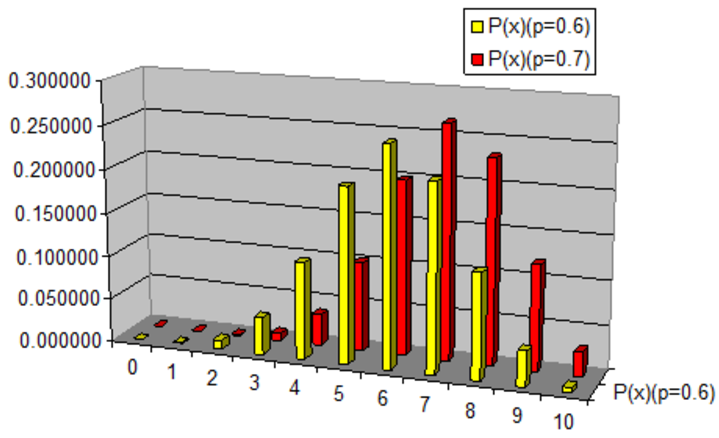
\includegraphics[width=0.5\linewidth]{images/estadistica9}
                      \label{fig:estadistica9}
                  \end{figure}
              \vspace{-0.23cm}
              La gráfica muestra que al aumentar la aceptación, la probabilidad máxima de compra se desplaza de 6 a 7 clientes.
          \end{frame}

          \begin{frame}{Distribución Hipergeométrica}
            Es similar a la binomial, pero con un tamaño de muestra grande en relación al tamaño de la población.
          \end{frame}

          \begin{frame}{Distribución De Poisson}
              Una variable de tipo Poisson cuenta el número de sucesos por unidad de tiempo, área, volumen, etc.  El experimento que la genera debe cumplir las siguientes condiciones:
              \begin{enumerate}
                  \item El número de éxitos que ocurren en cada región del tiempo o del espacio es independiente de lo que ocurra en cualquier otro tiempo o espacio disjunto del anterior.
                  \item La probabilidad de un‚ éxito en un tiempo o espacio pequeño es proporcional al tamaño de este y no depende de lo que ocurra fuera de él.
                  \item La probabilidad de encontrar uno o más‚ éxitos en una región del tiempo o del espacio tiende a cero a medida que se reducen las dimensiones de la región en estudio.
              \end{enumerate}
          $$ P(X=x)=\dfrac{e^{-\lambda}\lambda^x}{x!} $$
          donde $x = 0, 1, 2, 3, ...$

          \end{frame}


    \subsection*{Distribuciones Continuas de Probabilidad}

      \begin{frame}{}
         \begin{center}
            \textbf{ \huge
               Distribuciones Continuas de Probabilidad}
         \end{center}
      \end{frame}


      \begin{frame}{Valores de la variable aleatoria }
          \begin{figure}
              \centering
              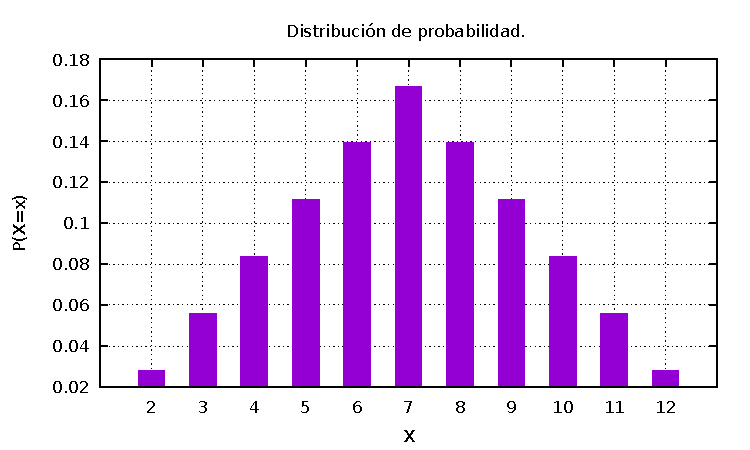
\includegraphics[width=0.5\linewidth]{images/p1}
          \end{figure}
          \pause
          \begin{itemize}
              \item Los datos que se colectan no sean completamente exactos
              \item Datos distribuidos, datos de forma discreta
              \item Se trabaja en intervalos
          \end{itemize}
          \pause
          Sin embargo, se pueden realizar aproximaciones y describir la probabilidad asociada a los valores de la variable aleatoria utilizando de modelos teóricos de probabilidad cuya gráfica es una línea continua.
      \end{frame}

      \begin{frame}{Distribuciones Continuas de Probabilidad}
          \begin{figure}
              \centering
              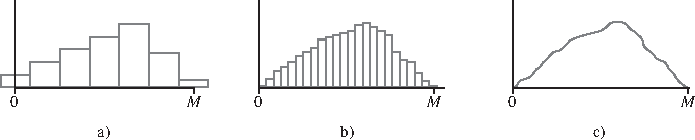
\includegraphics[width=0.7\linewidth]{images/estadistica10}
              \label{fig:estadistica10}
          \end{figure}

      \end{frame}

      \begin{frame}{Distribuciones Continuas de Probabilidad}

        \begin{block}{Distribuciones Continuas de Probabilidad}
          \begin{itemize}
            \item Normal
            \item Chi cuadrada
            \item F de Fisher
            \item Uniforme *
            \item Exponencial *
          \end{itemize}
        ´\end{block}
      \end{frame}

      \begin{frame}{DCP. Distribución Normal}
          La distribución normal es la más importante en toda la probabilidad y estadística. Muchas poblaciones numéricas tienen distribuciones que pueden ser representadas muy fielmente por
una curva normal apropiada.
          \pause
          \begin{block}{Distribuci\'on Normal}
            Se dice que una variable aleatoria continua $X$ tiene una distribución normal con parámetros $\mu$ y $\sigma$ (o $\mu$ y $\sigma^2$ ), donde $-\infty < \mu < \infty$ y $\sigma > 0$ o, si la función de densidad de
probabilidad de $X$ es:
            \pause
            $$f(x; \mu,\sigma) = \dfrac{1}{\sigma\sqrt{2\pi}} \exp^{-\dfrac{(x-\mu)^2}{2\sigma^2}} ,\quad -\infty < x < \infty$$
            $$e: 2.71828$$
            $$\pi: 3.14159$$
          \end{block}
      \end{frame}

      \begin{frame}{DCP. Distribución Normal. Propiedades}
          \begin{figure}
              \centering
              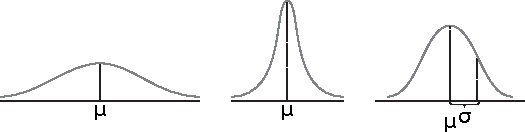
\includegraphics[width=0.7\linewidth]{images/estadistica11}
              \label{fig:estadistica11}
          \end{figure}

          \begin{block}{Distribuci\'on Normal}
              \begin{itemize}
                  \item $\mu$: es el valor medio de la distribución y es precisamente donde se sitúa el centro de la curva (de la campana de Gauss).
                  \item $\sigma^2$: es la varianza. Indica si los valores están más o menos alejados del valor central: si la varianza es baja los valores están próximos a la media; si es alta, entonces los valores están muy dispersos.
              \end{itemize}
          \end{block}
      \end{frame}

      \begin{frame}{DCP. Distribución Normal. Propiedades}
          \begin{figure}
              \centering
              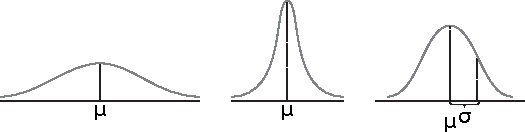
\includegraphics[width=0.55\linewidth]{images/estadistica11}
              \label{fig:estadistica11}
          \end{figure}

          \begin{block}{Distribuci\'on Normal}
             \begin{enumerate}
                 \item Los valores de la curva son positivos.
                 \item La curva es simétrica con respecto al valor de la media.
                 \item La curva tiene un valor máximo en el valor de la media.
                 \item La curva tiene puntos de inflexión en aquellos valores de x para los cuales a la media se le suma o se le resta una desviación estándar.
                 \item La curva, en sus extremos izquierdo y derecho, tiende a acercarse infinitamente al valor cero, es decir, el eje de las abscisas es asíntota horizontal.
                 \item El área bajo la curva es la unidad.
             \end{enumerate}
          \end{block}
      \end{frame}

      \begin{frame}{Distribución normal estándar o Distribución normal tipificada}
        \begin{block}{Distribución normal estándar}
          La distribución normal con valores de parámetro $\mu = 0$ y $\sigma = 1$ se llama \textbf{distribución normal estándar}. Una variable aleatoria que tiene una distribución normal estándar se llama \textbf{variable aleatoria normal estándar} y se denotará por $Z$. La función
de densidad de probabilidad de $Z$ es:
           $$f(z; 0, 1) = \dfrac{1}{\sqrt{2\pi}} \exp^{\dfrac{-z^2}{2}} ,\quad -\infty < z < \infty$$
           La gráfica de $f(z; 0, 1)$ se llama \textbf{\textit{curva normal estándar}}. La función de distribución acumulativa de $Z$ es $P(Z\leq z) = \Phi(z)$.
        \end{block}
        Con esta expresión se calcul\'o de forma numérica la tabla de frecuencias, con la cual vamos a trabajar a continuación.
      \end{frame}

      \begin{frame}{Distribución normal estándar o Distribución normal tipificada}
          \begin{block}{¿Cómo utilizar la tabla?}
              La columna de la izquierda indica el valor cuya probabilidad acumulada queremos conocer (x). La primera fila nos indica el segundo decimal del valor que estamos consultando, tolerancia para el calculo de error, vamos a tomar 0.05 (pues es el m\'as común).
          \end{block}
          \begin{block}{Ejemplo}
              Determínense las siguientes probabilidades normales estándar:
              \begin{itemize}
                  \item[a] $P(Z \leq 1.25)$
                  \item[b] $P(Z >
1.25)$
                  \item[c] $P(Z \leq -1.25)$
                  \item[d] $P(-0.38 \leq Z \leq 1.25)$
              \end{itemize}
          \end{block}
      \end{frame}

      \begin{frame}{El ejemplo}
          \begin{block}{Ejemplo}
              Determínense las siguientes probabilidades normales estándar:
              \begin{itemize}
                  \item[a] $P(Z \leq 1.25)$
                  \item[b] $P(Z >
1.25)$
                  \item[c] $P(Z \leq -1.25)$
                  \item[d] $P(-0.38 \leq Z \leq 1.25)$
              \end{itemize}
          \end{block}
          \begin{itemize}
              \item[a, b]
          \end{itemize}
          \begin{figure}
              \centering
              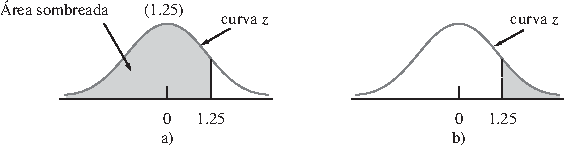
\includegraphics[width=1\linewidth]{images/estadistica12}
              \label{fig:estadistica12}
          \end{figure}

      \end{frame}
      \begin{frame}{El ejemplo}
          \begin{block}{Ejemplo}
              Determínense las siguientes probabilidades normales estándar:
              \begin{itemize}
                  \item[a] $P(Z \leq 1.25)$
                  \item[b] $P(Z >
1.25)$
                  \item[c] $P(Z \leq -1.25)$
                  \item[d] $P(-0.38 \leq Z \leq 1.25)$
              \end{itemize}
          \end{block}
          \begin{itemize}
              \item[c, d]
          \end{itemize}
          \begin{figure}
              \centering
              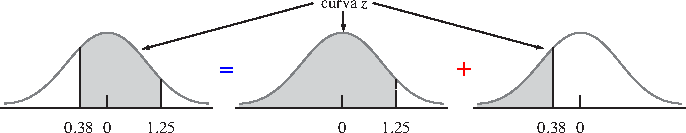
\includegraphics[width=1\linewidth]{images/estadistica13}
              \label{fig:estadistica12}
          \end{figure}

      \end{frame}

      \begin{frame}{Ejercicio 1}
          \begin{block}{Ejercicio 1}
              \begin{itemize}
                  \item Busque en la tabla las probabilidades acumuladas hasta los valores 0.71, 1.83, 2.25
                  \item Halle los valores de X que corresponden a probabilidades acumuladas de 0.75, 0.80, 0.90 y 0.95.
              \end{itemize}
          \end{block}
      \end{frame}


      \subsubsection*{$\sigma^2$}
        \begin{frame}{}
\begin{center}
    \textbf{            \huge Distribución $\sigma^2$}
\end{center}
        \end{frame}

    \subsection*{Distribuciones Muestrales}
    \begin{frame}{title}
        \begin{block}{title}
            content...
        \end{block}
    \end{frame}


\end{document}